\documentclass[12pt]{article}
\usepackage{amsmath}
\usepackage{amssymb}
\usepackage{geometry}
\usepackage{amsmath, amsfonts, bm, graphicx}
\usepackage{tabularx}
\usepackage{booktabs} 
\usepackage{float}
\usepackage{enumitem}
\geometry{margin=1in}

\title{}
\date{}
\author{}

\begin{document}
\subsection*{\boxed{\text{HW 2 - Zeshui Song}}}

\section*{3.21}
\vspace{-3.5em}
\begin{figure}[H]
    \centering
    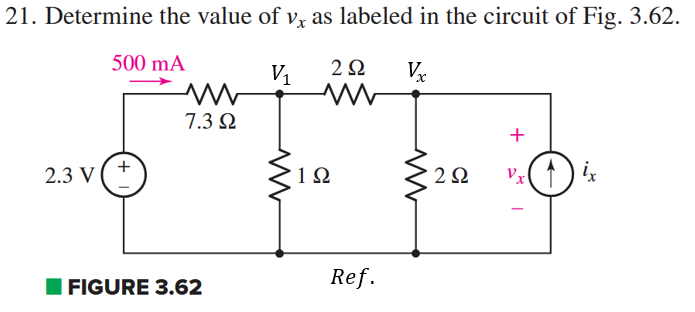
\includegraphics[width=0.8\textwidth]{3-21.png}
\end{figure}
\vspace{-1em}
Using nodal analysis, assigning $V_1$ and $V_x$, I can apply KCL at node 1:
\[[500\times10^{-3}\,\text{A}] = \frac{V_1}{[1\,\Omega]}+\frac{V_1-V_x}{[2\,\Omega]}\]
Using KVL (CCW) starting from negative terminal of the voltage source around the left loop to find $V_1$:
\[[2.3\,\text{V}]-[500\times10^{-3}\,\text{A}][7.3\,\Omega]-V_1=0\]
\[V_1 = -1.35\,\text{V}\]
Plugging in $V_1$ into the KCL equation to find $V_x$:
\[[500\times10^{-3}\,\text{A}] = \frac{[-1.35\,\text{V}]}{[1\,\Omega]}+\frac{[-1.35\,\text{V}]-V_x}{[2\,\Omega]}\]
\[\boxed{V_x = -5.05\,\text{V}}\]

\section*{3.23}
\vspace{-3.5em}
\begin{figure}[H]
    \centering
    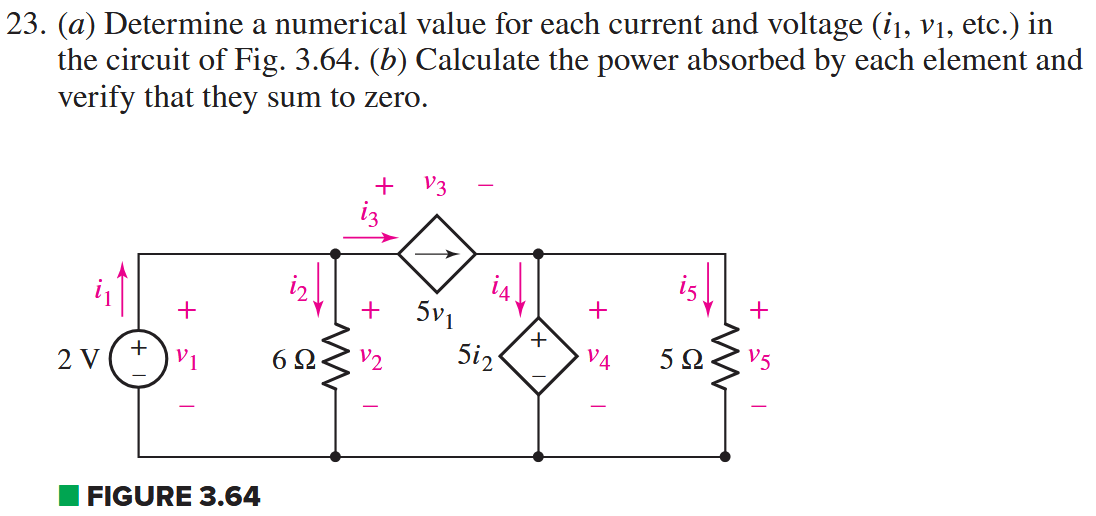
\includegraphics[width=0.8\textwidth]{3-23.png}
\end{figure}
\vspace{-1em}
\textbf{(a)}\\
$i_2$ and $v_2$: KVL (CCW) starting from negative terminal of the 2V source around the left loop:
\[[2\,\text{V}]-i_2[6\,\Omega]=0 \quad \implies i_2 = 0.33\,\text{A}\]
\[[2\,\text{V}]-v_2=0 \quad \implies v_2 = 2\,\text{V}\]
$i_3$ and $v_4$ by plugging in for $v_1$ and $i_2$:
\[i_3 = 5v_1 = 5[2\,\text{V}] = 10\,\text{A}\]
\[v_4 = 5i_2 = 5[0.33\,\text{A}] = 1.67\,\text{V}\]
$i_1$ by KCL at top node of $6\,\Omega$ resistor:
\[i_1 = i_2 + i_3 = [0.33\,\text{A}]+[10\,\text{A}] = 10.33\,\text{A}\]
$v_3$ by KVL (CCW) starting from negative terminal of the $6\,\Omega$ resistor around the middle loop:
\[v_2-v_3-v_4=0 \quad \implies v_3 = [2\,\text{V}]-[1.67\,\text{V}] = 0.33\,\text{V}\]
$v_5$ is in parallel with $v_4$, thus it has the same voltage:
\[v_5 = v_4 = 1.67\,\text{V}\]
$i_5$ by Ohm's law:
\[i_5 = \frac{[1.67\,\text{V}]}{[5\,\Omega]} = 0.334\,\text{A}\]
Lastly, $i_4$ by KCL at top node of $v_4$:
\[i_3 = i_4 + i_5 \quad \implies i_4 = i_3 - i_5 = [10\,\text{A}] - [0.334\,\text{A}] = 9.666\,\text{A}\]

\begin{table}[H]
\centering
\renewcommand{\arraystretch}{1.5}
\begin{tabular}{|l|c|c|}
\hline
\textbf{Element} & \textbf{Voltage, $v$ [V]} & \textbf{Current, $i$ [A]} \\ \hline
2V Source &$v_1=$ 2 &$i_1=$ 10.33 \\ \hline
6 $\Omega$ Resistor &$v_2=$ 2 &$i_2=$ 0.33 \\ \hline
Dependent $5v_1$ &$v_3=$ 0.33 &$i_3=$ 10 \\ \hline
Dependent $5i_2$ &$v_4=$ 1.67 &$i_4=$ 9.66 \\ \hline
5 $\Omega$ Resistor &$v_5=$ 1.67 &$i_5=$ 0.33 \\ \hline
\end{tabular}
\end{table}\newpage\noindent\vspace{-2em}
\textbf{(b)}
\begin{table}[H]
\centering
\renewcommand{\arraystretch}{1.5} 
\begin{tabular}{|l|c|c|c|}
\hline
\textbf{Element} & \textbf{Voltage, $v$ [V]} & \textbf{Current, $i$ [A]} & \textbf{$P=Vi$ [W]} \\ \hline
2V Source & $v_1=2$ & $i_1=10.33$ & $P_1 = -20.66$ \\ \hline
6 $\Omega$ Resistor & $v_2=2$ & $i_2=0.33$ & $P_2 = 0.66$ \\ \hline
Dependent $5v_1$ & $v_3=0.33$ & $i_3=10$ & $P_3 = 3.30$ \\ \hline
Dependent $5i_2$ & $v_4=1.67$ & $i_4=9.66$ & $P_4 = 16.13$ \\ \hline
5 $\Omega$ Resistor & $v_5=1.67$ & $i_5=0.33$ & $P_5 = 0.55$ \\ \hline
\multicolumn{3}{|l|}{\textbf{Total Power Absorbed} (Not exactly 0 b/c of rounding)} & \textbf{-0.02} \\ \hline
\end{tabular}
\end{table}\noindent
\underline{Note:} The sign convention for power \textit{absorbed} is negative for sources (current enters - and leaves + terminal) and positive for loads (current enters + and leaves - terminal).

\section*{3.34}
\vspace{-3.5em}
\begin{figure}[H]
    \centering
    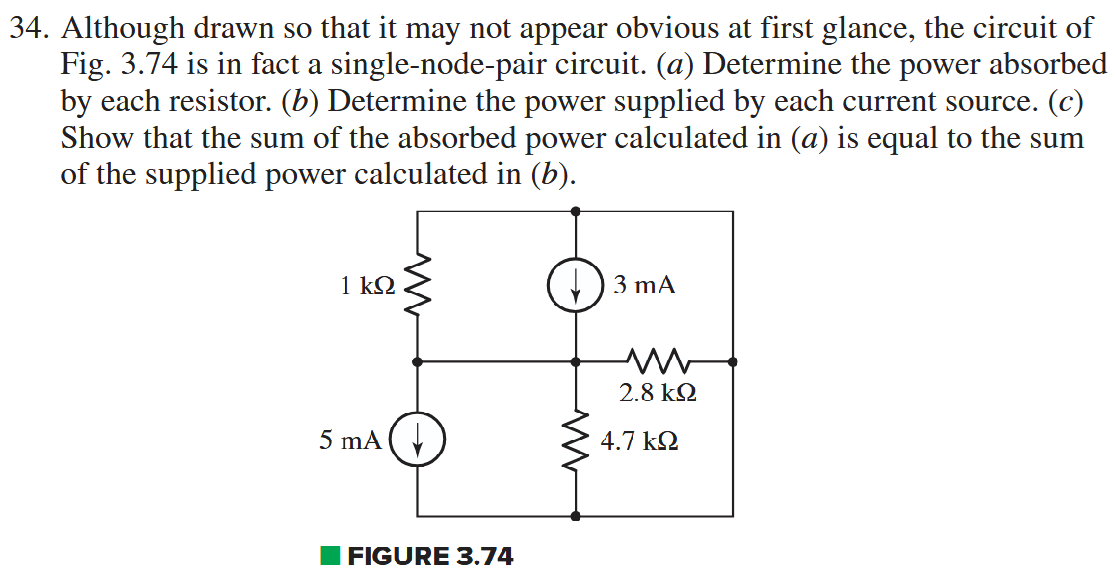
\includegraphics[width=0.8\textwidth]{3-34.png}
\end{figure}
\vspace{-1em}
This is a \textbf{single-node pair circuit} meaning that every element is in parallel across the same two nodes. Thus, it can be redrawn:
\begin{figure}[H]
    \centering
    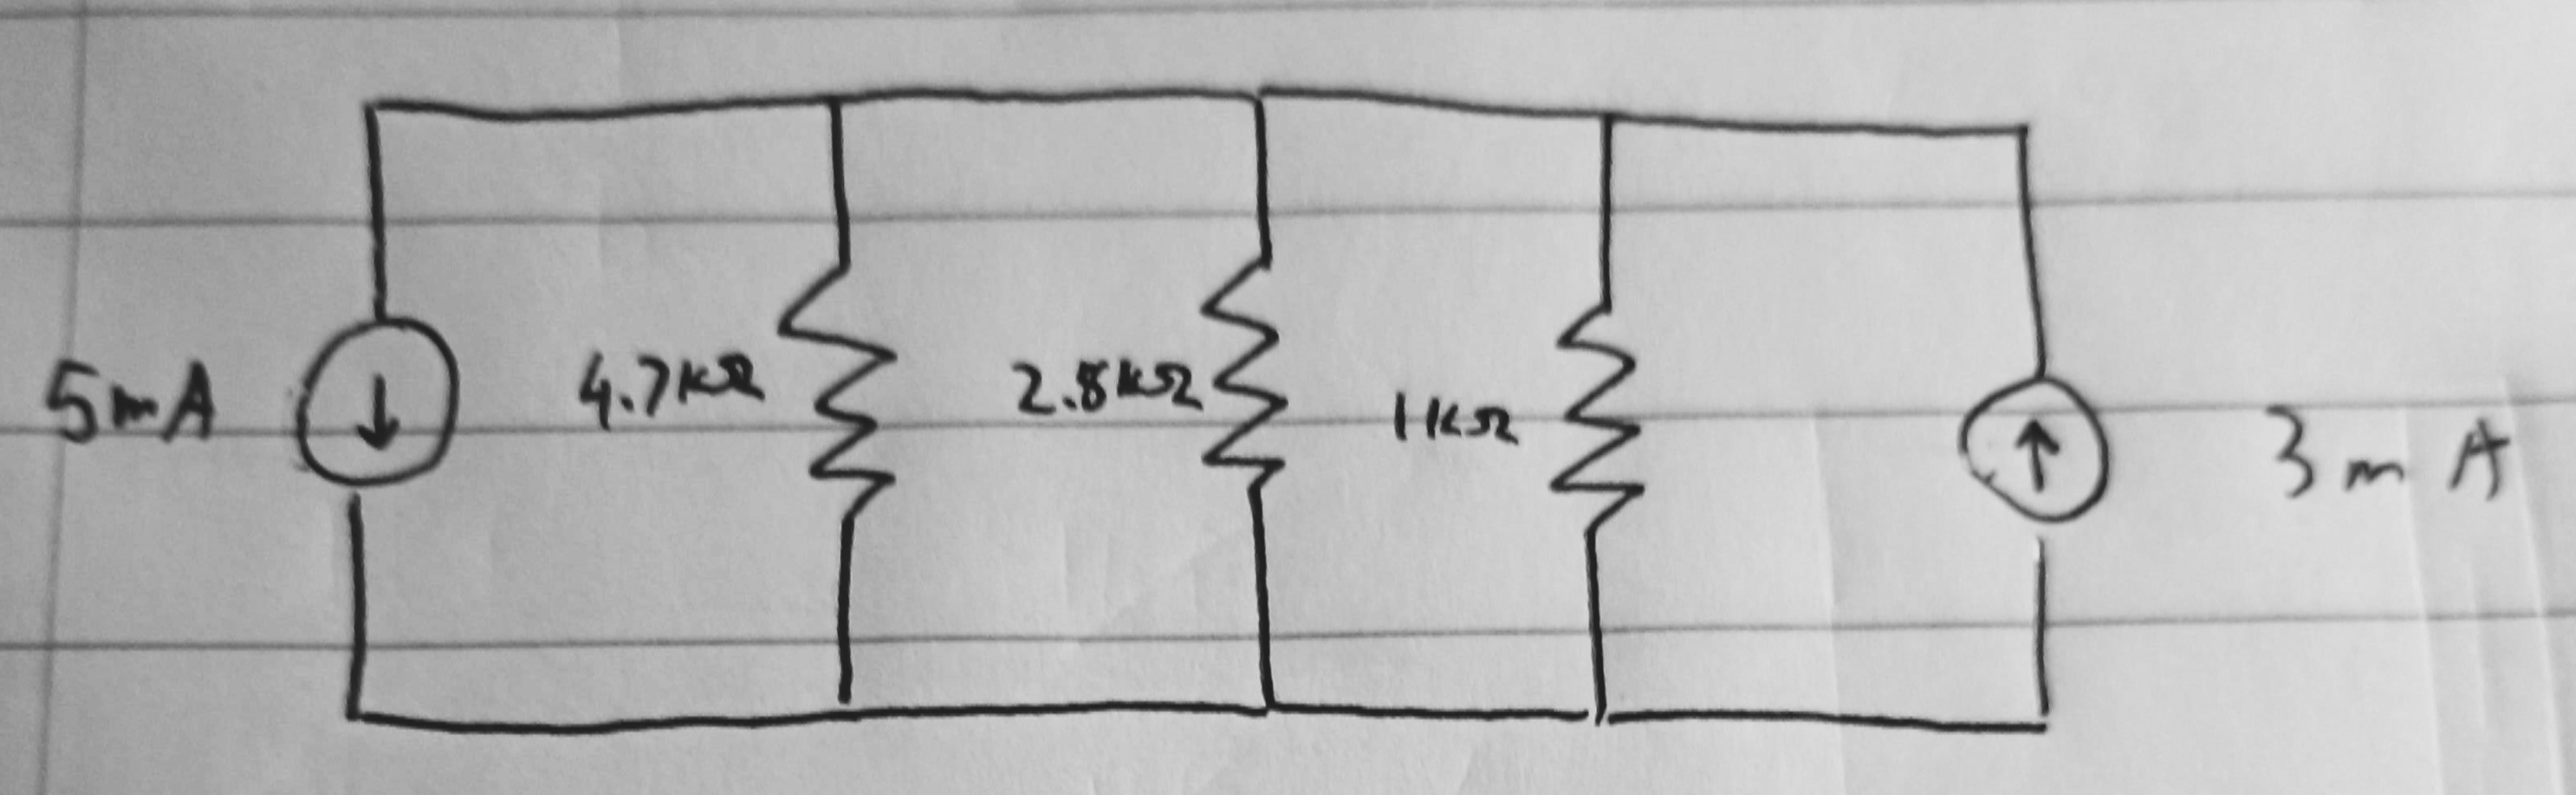
\includegraphics[width=0.8\textwidth]{3-34_1.jpg}
\end{figure}\vspace{-1em}\noindent
\underline{Note:} The direction of the current sources has to be consistent with the direction in which they feed into/out of the resistors.
\textbf{(a)} We can further simplify by combining the resistors in parallel:
\[\frac{1}{R_{eq}} = \frac{1}{[4.7\times10^3\,\Omega]} + \frac{1}{[2.8\times10^3\,\Omega]} + \frac{1}{[1\times10^3\,\Omega]}
\quad \implies R_{eq} = 636.979\,\Omega\]
\begin{figure}[H]
    \centering
    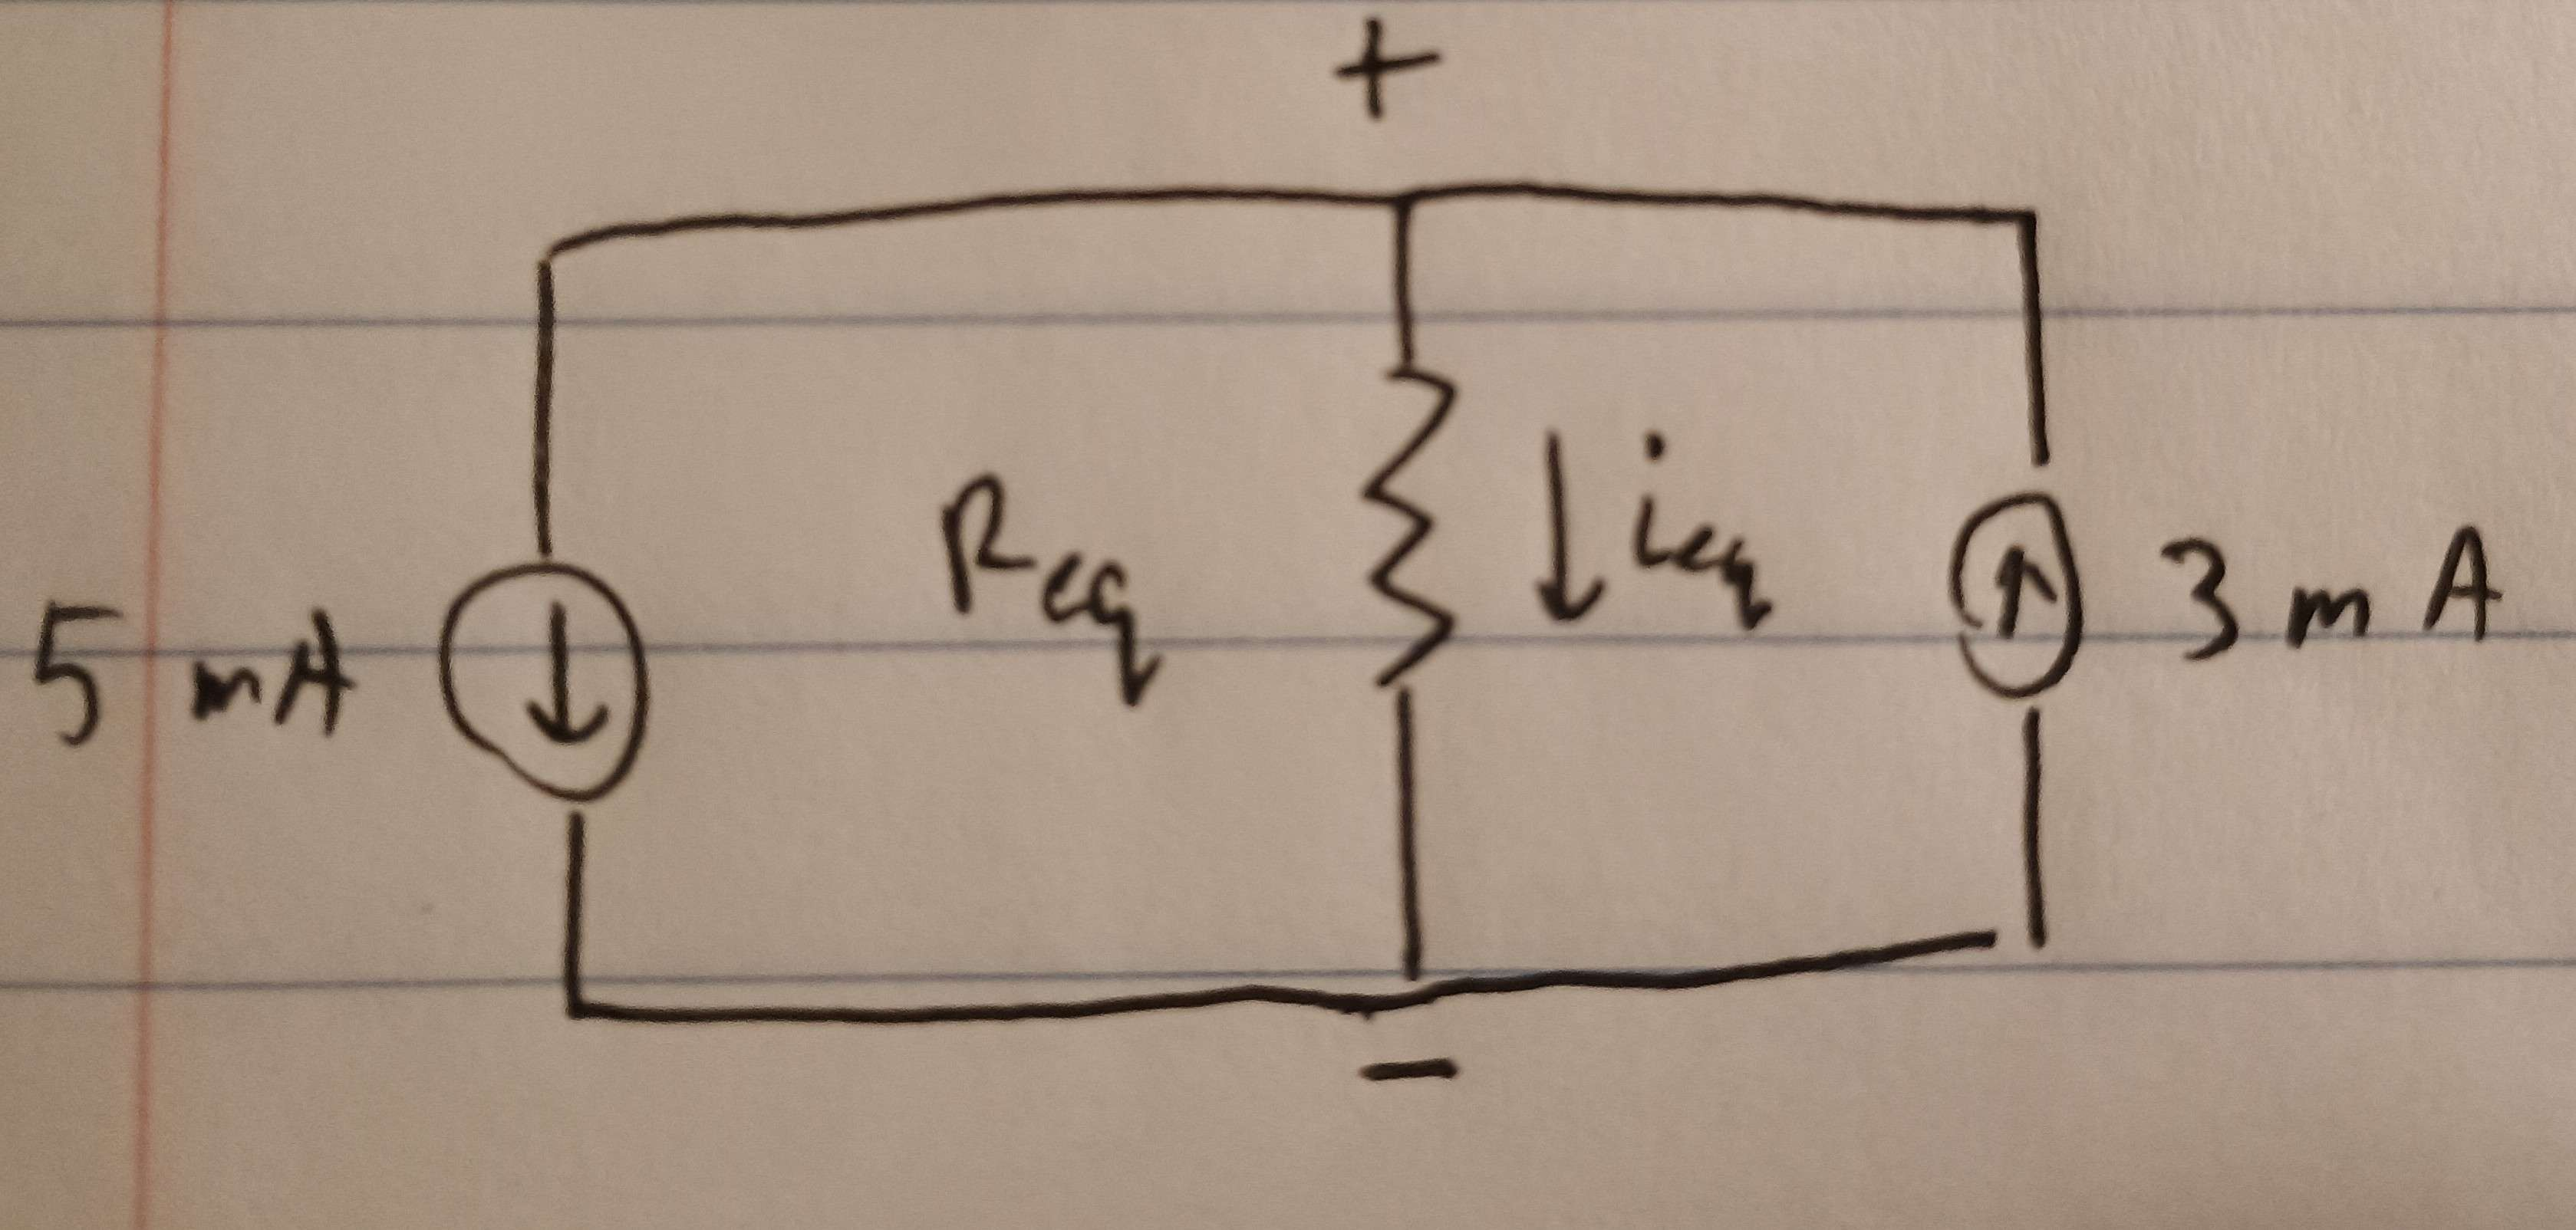
\includegraphics[width=0.5\textwidth]{3-34_2.jpg}
\end{figure}\noindent
Using KCL at the top node:
\[i_{\text{eq}} = [3\times10^{-3}\,\text{A}]-[5\times10^{-3}\,\text{A}] = -2\times10^{-3}\,\text{A}\]
By Ohm's law:
\[V = [(-2\times10^{-3}\,\text{A})][636.979\,\Omega] = -1.2739\,\text{V}\]
\begin{table}[H]
\centering
\renewcommand{\arraystretch}{1.5} 
\begin{tabular}{|l|c|c|c|}
\hline
\textbf{Element} & \textbf{Voltage, $v$ [V]} & \textbf{Current, $i=V/R$ [A]} & \textbf{$P=vi$ [W]} \\ \hline
5 mA Source & -1.2739 & $5\times10^{-3}$ & $-6.369\times10^{-3}$ \\ \hline
4.7 k$\Omega$ Resistor & -1.2739 & $-0.271\times10^{-3}$ & $.345\times10^{-3}$ \\ \hline
2.8 k$\Omega$ Resistor & -1.2739 & $-0.454\times10^{-3}$ & $0.578\times10^{-3}$ \\ \hline
1 k$\Omega$ Resistor & -1.2739 & $-1.273\times10^{-3}$ & $1.621\times10^{-3}$ \\ \hline
3 mA Source & -1.2739 & $-3\times10^{-3}$ & $3.821\times10^{-3}$ \\ \hline
\multicolumn{3}{|l|}{\textbf{Total Power Absorbed} (Not exactly 0 b/c of rounding)} & \textbf{-0.004} \\ \hline
\end{tabular}
\end{table}\noindent
\underline{Note:} I had previously defined the positive voltage and current to be top to down, which is why everything turned out negative, except for the current from the 5 mA source.

\section*{3.38}
\vspace{-3.5em}
\begin{figure}[H]
    \centering
    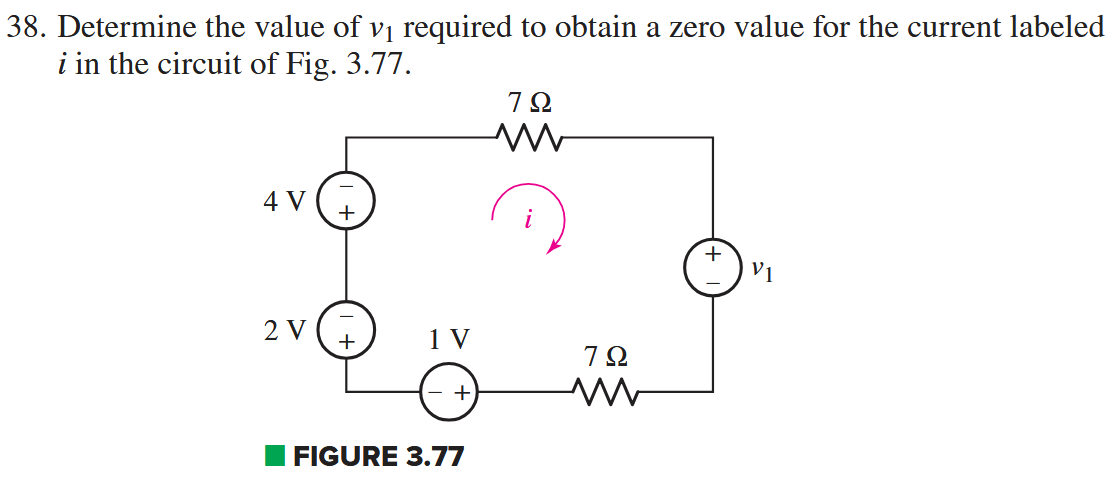
\includegraphics[width=0.8\textwidth]{3-38.png}
\end{figure}
\vspace{-1em}
Using KVL (CCW) starting from the positive terminal of the 2 V source around the loop:
\[-[2\,\text{V}]-[4\,\text{V}]-i\cdot[7\,\Omega]-v_1-i\cdot[7\,\Omega]-[1\,\text{V}]=0\]
Since $i=0$, we have:
\[-[2\,\text{V}]-[4\,\text{V}]-v_1-[1\,\text{V}]=0 \quad \implies \quad \boxed{v_1 = -7\,\text{V}}\]

\section*{3.39}
\vspace{-3.5em}
\begin{figure}[H]
    \centering
    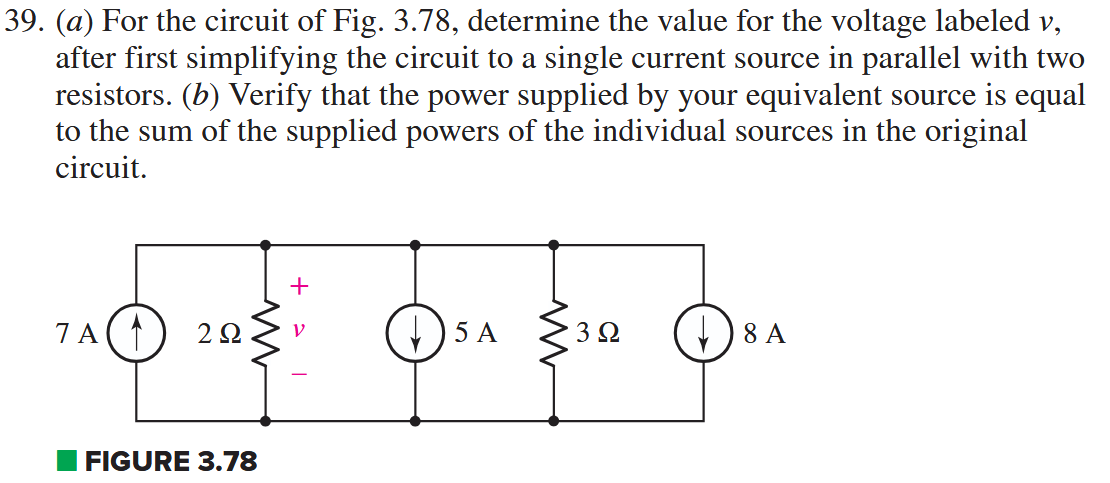
\includegraphics[width=0.8\textwidth]{3-39.png}
\end{figure}
\vspace{-1em}
\textbf{(a)} 
Similar to problem \textit{3.34}, if I combine the resistors in parallel, I can use KCL at the top node to find $i_{\text{eq}}$, and thus an equivalent current source and resistor in parallel:
\[i_{\text{eq}}=[7\,\text{A}]-[5\,\text{A}]-[8\,\text{A}]=-6\,\text{A}\]
\[R_{\text{eq}} = \frac{[2\,\Omega]\cdot[3\,\Omega]}{[2\,\Omega]+[3\,\Omega]} = 1.2\,\Omega\]
Thus, the voltage across each element is:
\[v = [(-6\,\text{A})][1.2\,\Omega] = \boxed{-7.2\,\text{V}}\]
\vspace{-2em}
\begin{figure}[H]
    \centering
    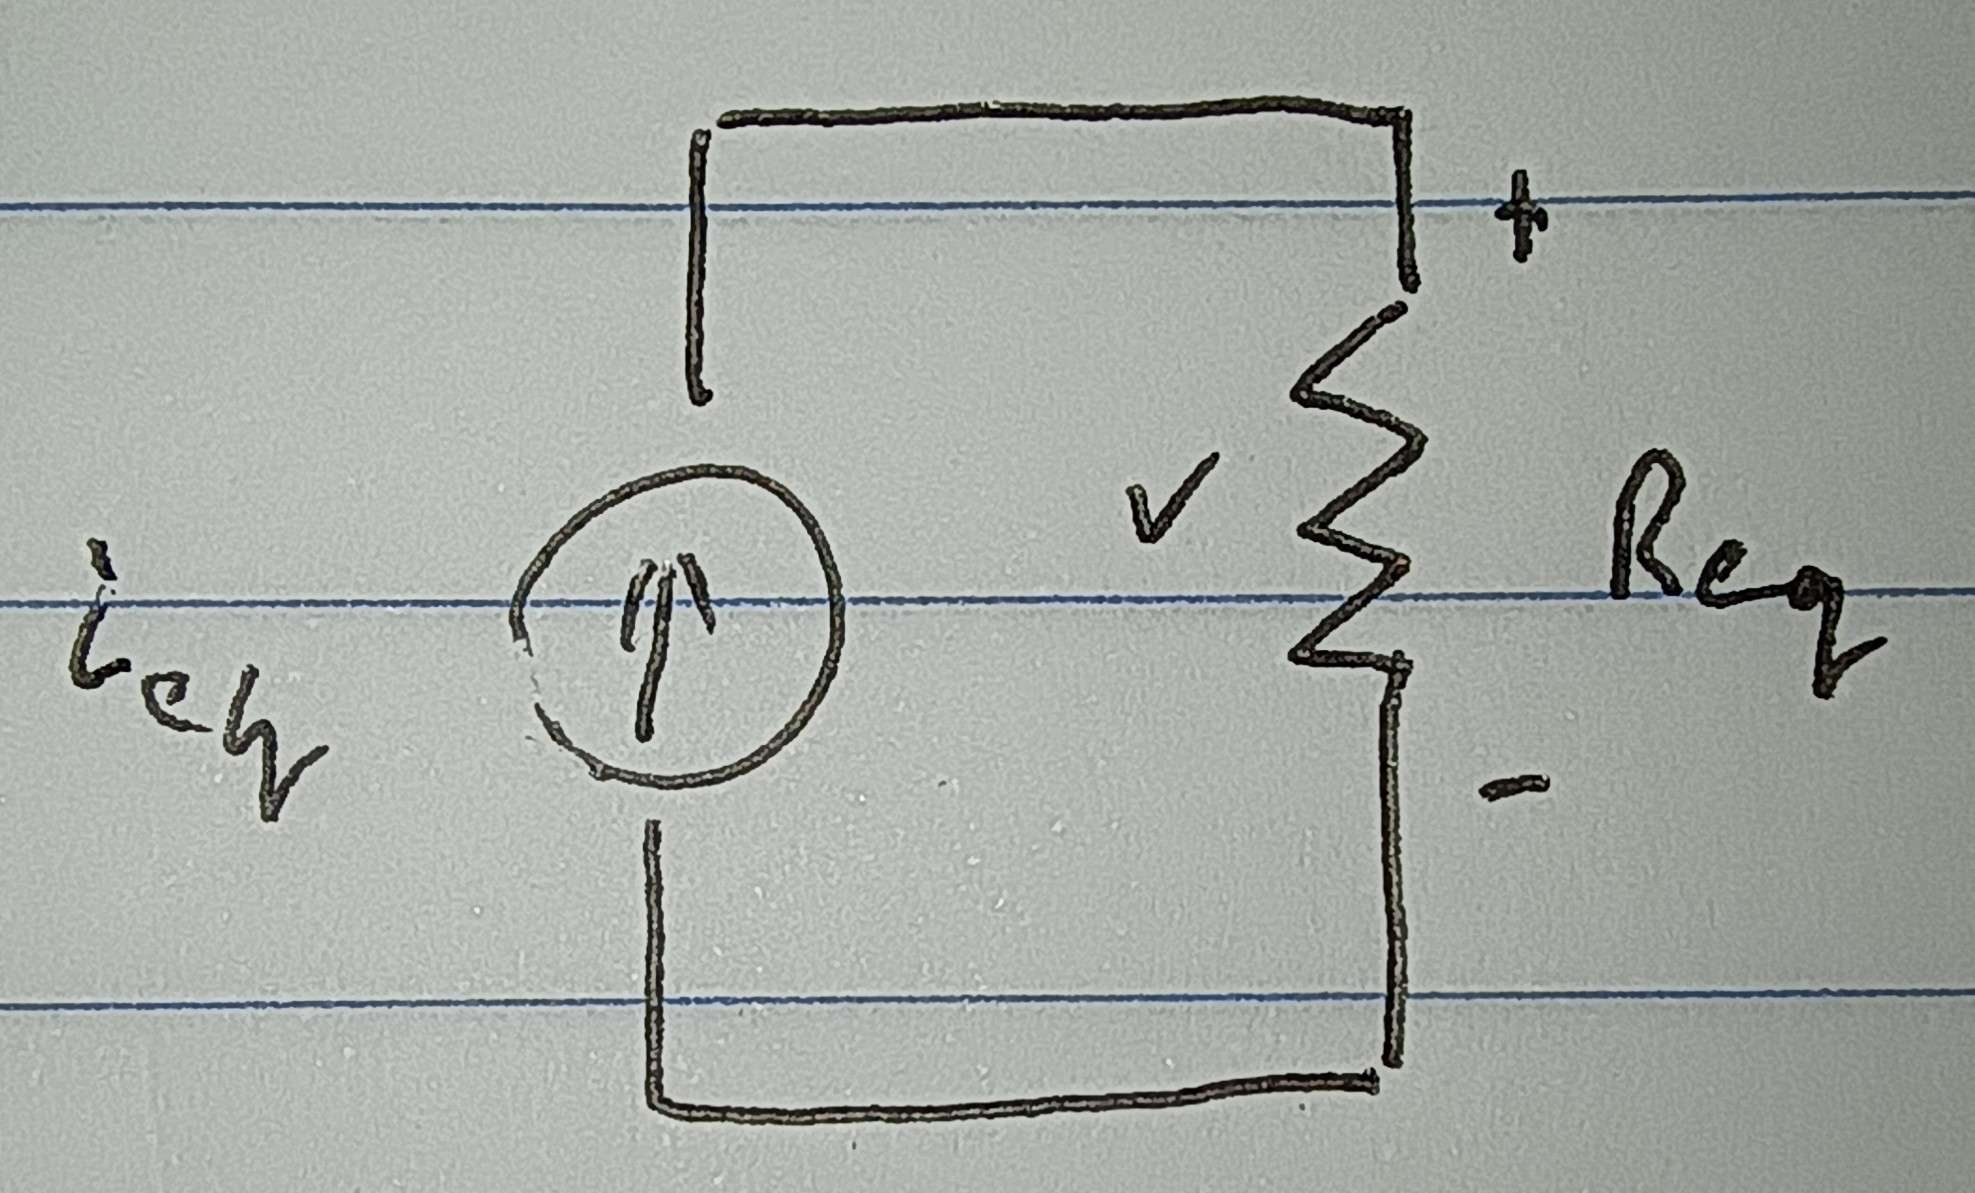
\includegraphics[width=0.4\textwidth]{3-39_1.jpg}
\end{figure}\noindent
\textbf{(b)} Since the voltage $v$ supplied by each current source is the same, the power supplied by each current source is then dependent only on the current supplied (following the sign convention for positive voltage and current):
\[P_{\text{7 A}} = [-7.2\,\text{V}]\cdot[7\,\text{A}] = -50.4\,\text{W}\]
\[P_{\text{5 A}} = [-7.2\,\text{V}]\cdot[-5\,\text{A}] = 36\,\text{W}\]
\[P_{\text{8 A}} = [-7.2\,\text{V}]\cdot[-8\,\text{A}] = 57.6\,\text{W}\]
\[\implies \boxed{\sum P = 43.2\,\text{W}}\]
For the equivalent current source:
\[P_{\text{eq}} = [-7.2\,\text{V}]\cdot[-6\,\text{A}] = \boxed{43.2\,\text{W}}\]

\section*{3.43}
\vspace{-3.5em}
\begin{figure}[H]
    \centering
    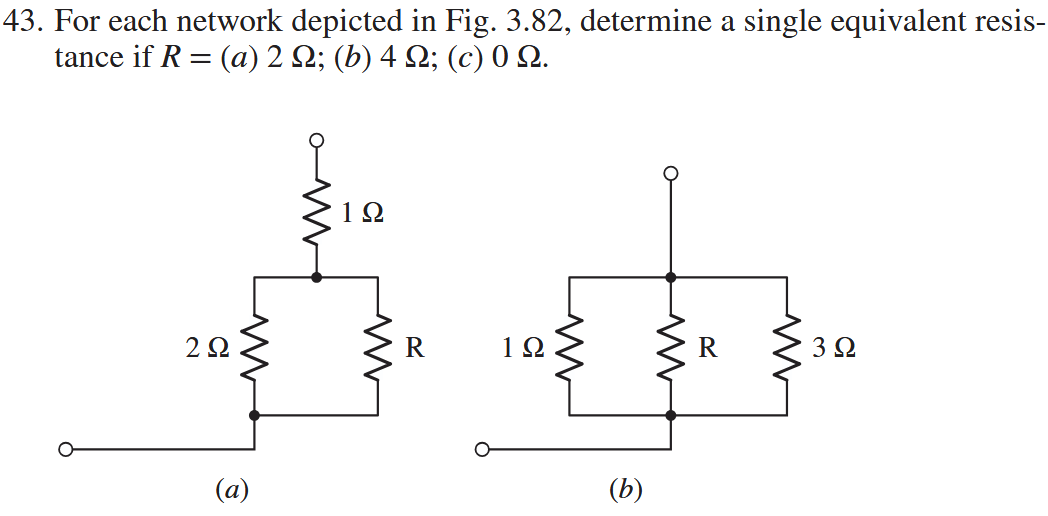
\includegraphics[width=0.8\textwidth]{3-43.png}
\end{figure}
\vspace{-1em}
\textbf{(a)}\\
    Combine the resistors in parallel:
    \[R_{\parallel} = \frac{[2\,\Omega]\cdot R}{[2\,\Omega]+R}\]
    Combine with the series resistor:
    \[R_{\text{eq}} = [1\,\Omega] + R_{\parallel} = 1 + \frac{2R}{2+R}\]
\begin{enumerate}[label=(\roman*)]
    \item $R=2\,\Omega$: \[R_{\text{eq}} = 1 + \frac{2R}{2+R} = \boxed{2\,\Omega}\]
    \item $R=4\,\Omega$: \[R_{\text{eq}} = 1 + \frac{2R}{2+R} = \boxed{2.33\,\Omega}\]
    \item $R=0\,\Omega$: \[R_{\text{eq}} = 1 + \frac{2R}{2+R} = \boxed{1\,\Omega}\]
\end{enumerate}
\textbf{(b)}\\
Combine the resistors in parallel:
    \[\frac{1}{R_{\text{eq}}} = \frac{1}{[1\,\Omega]} + \frac{1}{[R\,\Omega]} + \frac{1}{[3\,\Omega]} \quad \implies R_{\text{eq}} = \frac{3R}{4R+3}\]
\begin{enumerate}[label=(\roman*)]
    \item $R=2\,\Omega$: \[R_{\text{eq}} = \frac{3R}{4R+3} = \boxed{0.5454\,\Omega}\]
    \item $R=4\,\Omega$: \[R_{\text{eq}} = \frac{3R}{4R+3} = \boxed{0.6315\,\Omega}\]
    \item $R=0\,\Omega$: \[R_{\text{eq}} = \frac{3R}{4R+3} = \boxed{0\,\Omega}\]
\end{enumerate}

\section*{3.46}
\vspace{-3.5em}
\begin{figure}[H]
    \centering
    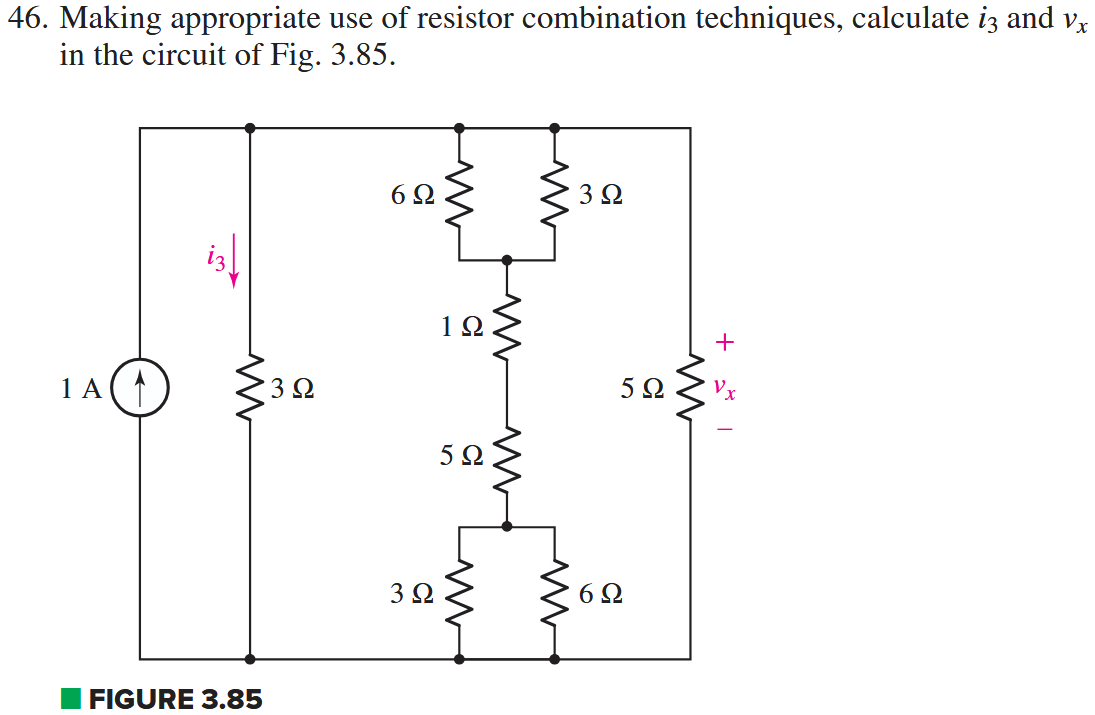
\includegraphics[width=0.8\textwidth]{3-46.png}
\end{figure}
\vspace{-1em}
Combine $3\,\Omega$ and $6\,\Omega$ resistors in parallel:
\[\frac{[3\,\Omega]\cdot[6\,\Omega]}{[3\,\Omega]+[6\,\Omega]} = 2\,\Omega\]
Combine all resistors on the second branch in series:
\[[2\,\Omega] + [1\,\Omega] +[5\,\Omega] + [2\,\Omega] = 10\,\Omega\]
Now combine resistors in all 3 branches in parallel:
\[\frac{1}{R_{eq}} = \frac{1}{[3\,\Omega]} + \frac{1}{[10\,\Omega]} + \frac{1}{[5\,\Omega]} \quad \implies R_{eq} = 1.578\,\Omega\]
Using Ohm's law to find voltage across each branch:
\[V = [1\,\text{A}][1.578\,\Omega] = 1.578\,\text{V}\]
Thus:
\[v_3 = i_3 \cdot [3\,\Omega] = [1.578\,\text{V}] \quad \implies i_3 = \boxed{0.526\,\text{A}}\]
\[\boxed{v_x = 1.578\,\text{V}}\]

\section*{3.48}
\vspace{-3.5em}
\begin{figure}[H]
    \centering
    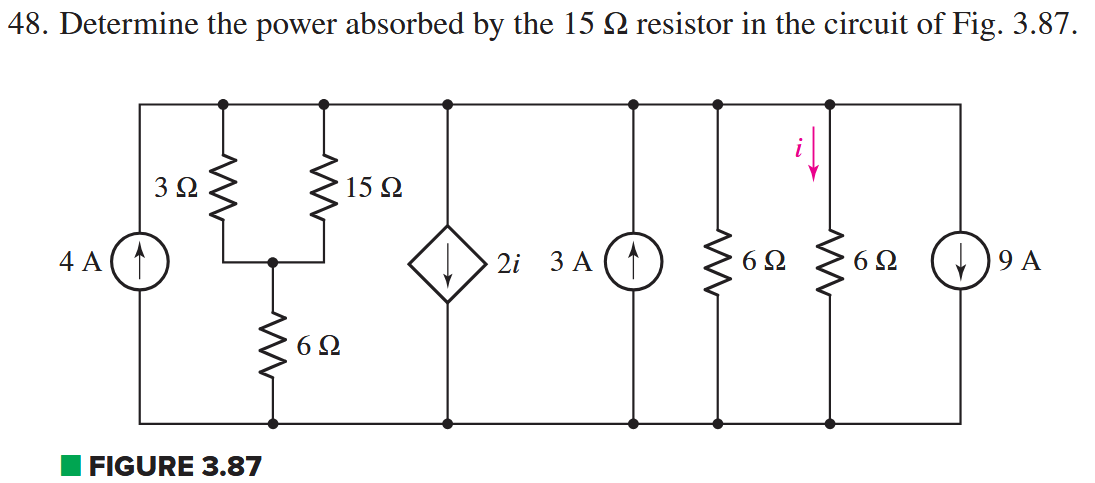
\includegraphics[width=0.8\textwidth]{3-48.png}
\end{figure}
\vspace{-1em}
First simplify the branch with the $3\,\Omega$, $15\,\Omega$, and $6\,\Omega$ resistors:
\[R = \frac{[3\,\Omega]\cdot[15\,\Omega]}{[3\,\Omega]+[15\,\Omega]} + [6\,\Omega] = 8.5\,\Omega\]
Apply Nodal analysis (all elements are in $\parallel$ so the node voltage is the same across all elements):
\begin{figure}[H]
    \centering
    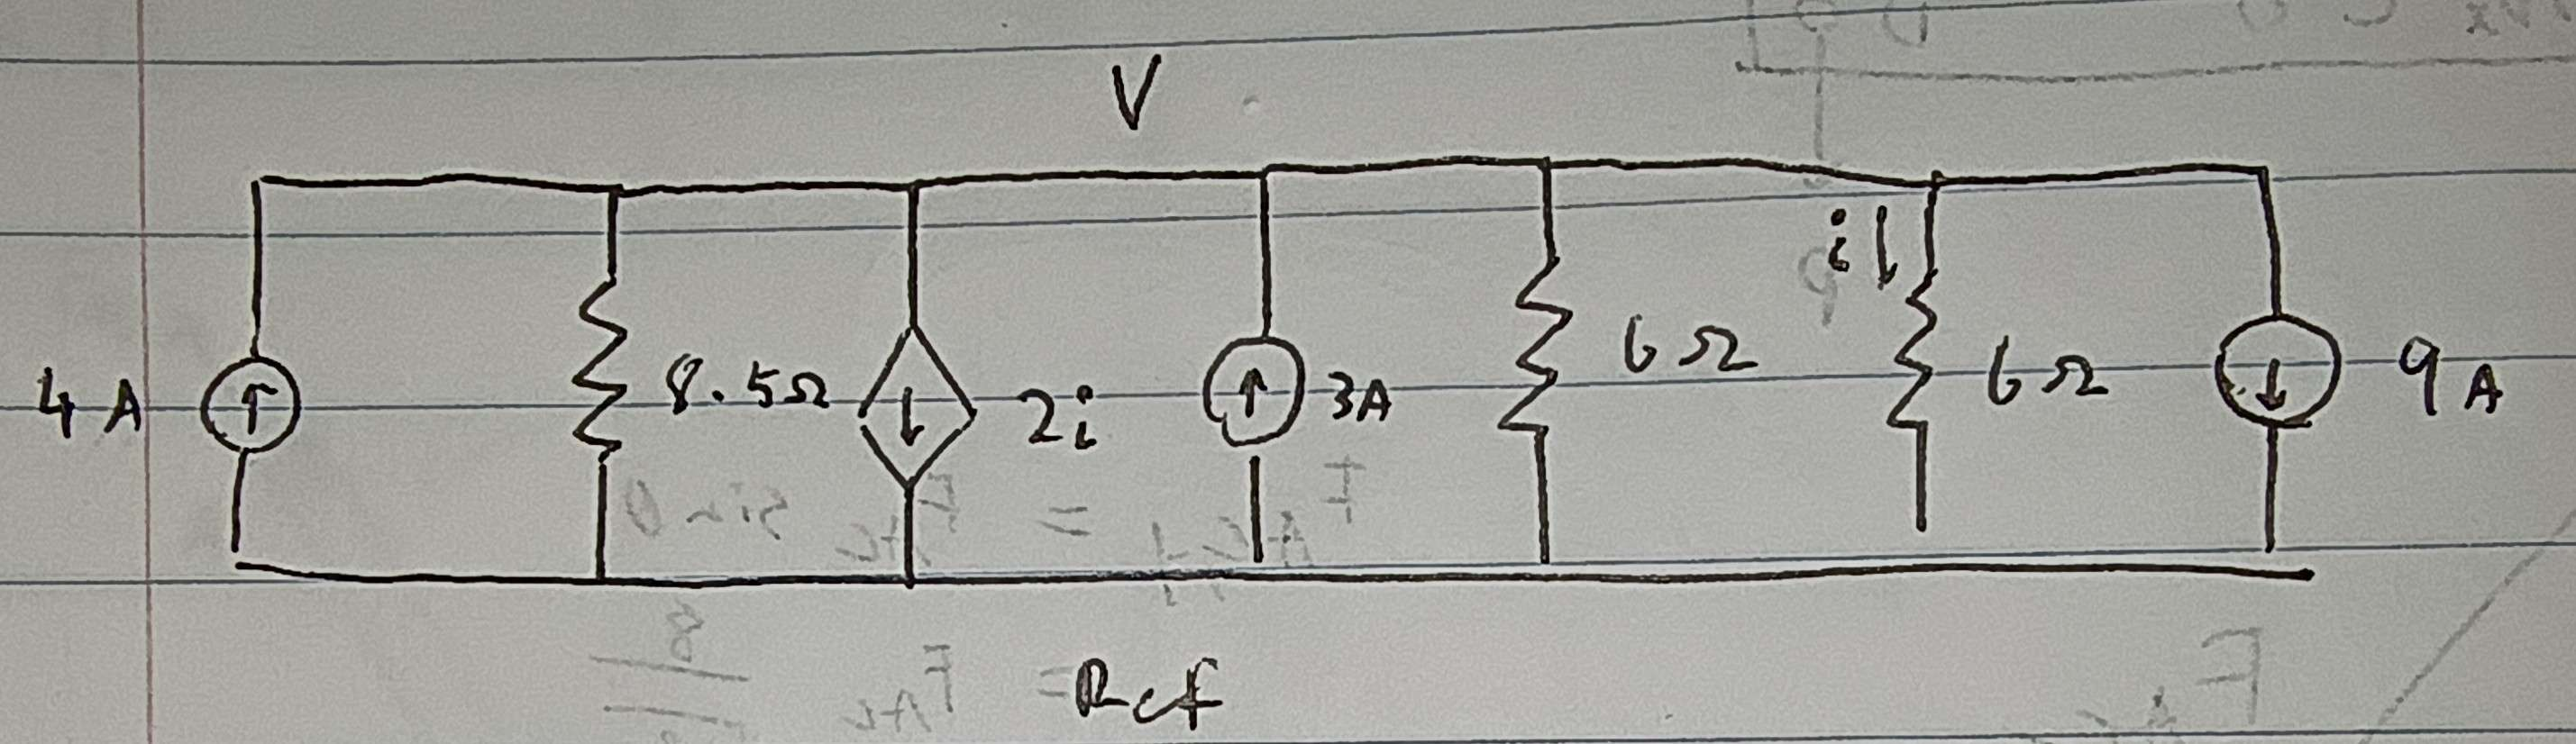
\includegraphics[width=0.8\textwidth]{3-48_1.jpg}
\end{figure}\noindent
KCL at top node of 3 A source:
\[[3\,\text{A}] = 2i - [4\,\text{A}]+[9\,\text{A}]+\frac{V}{[8.5\,\Omega]}+\frac{V}{[6\,\Omega]}+\frac{V}{[6\,\Omega]}\]
\[i = \frac{V}{[6\,\Omega]}\]
Thus, solving for $V$:
\[3=\frac{2V}{6}-4+9+\frac{V}{8.5}+\frac{V}{6}+\frac{V}{6} \quad \implies V = -2.55\,\text{V}\]
Using the voltage divider rule on the $8.5\,\Omega$ branch to find $v_{15}$ (which is the same as the $2.5\,\Omega$ parallel combination):
\[v_{2.5} = [-2.55\,\text{V}]\frac{[2.5\,\Omega]}{[8.5\,\Omega]} = -0.75\,\text{V}\]
The power absorbed by the $15\,\Omega$ resistor is then:
\[i_{15} = \frac{[-0.75\,\text{V}]}{[15\,\Omega]} = -0.05\,\text{A}\]
\[P_{15} = [-0.75\,\text{V}]\cdot[-0.05\,\text{A}] = \boxed{0.0375\,\text{W}}\]
\underline{Note:} The voltage divider rule applies to series elements, where 
\[v_x = V\frac{R_x}{R_{\text{total}}}\]

\section*{3.54}
\vspace{-3.5em}
\begin{figure}[H]
    \centering
    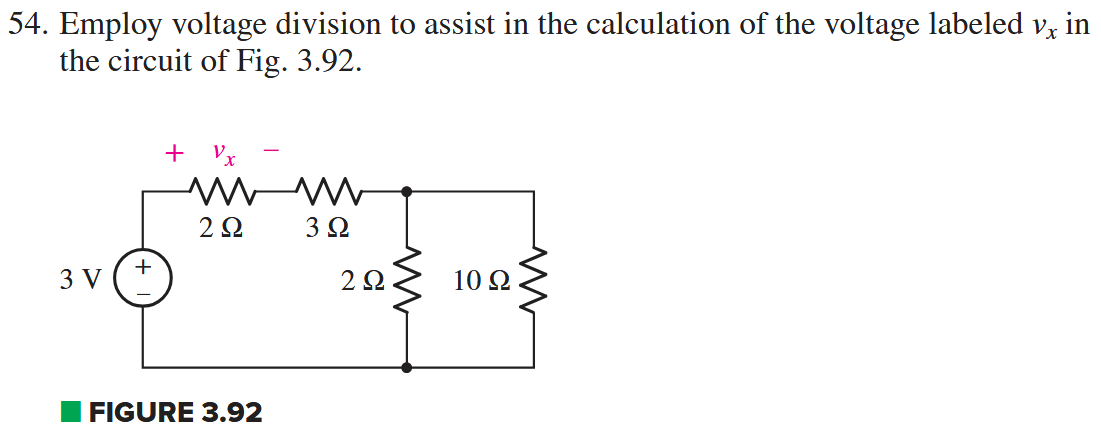
\includegraphics[width=0.8\textwidth]{3-54.png}
\end{figure}
\vspace{-1em}
Combine the $2\,\Omega$ and $10\,\Omega$ resistors in parallel:
\[R_{\parallel} = \frac{[2\,\Omega]\cdot[10\,\Omega]}{[2\,\Omega]+[10\,\Omega]} = 1.66\,\Omega\]
Use voltage divider rule to find $v_x$:
\[v_x = [3\,\text{V}]\frac{[2\,\Omega]}{[2\,\Omega]+[3\,\Omega]+[1.66\,\Omega]} = \boxed{0.692\,\text{V}}\]

\section*{3.56}
\vspace{-3.5em}
\begin{figure}[H]
    \centering
    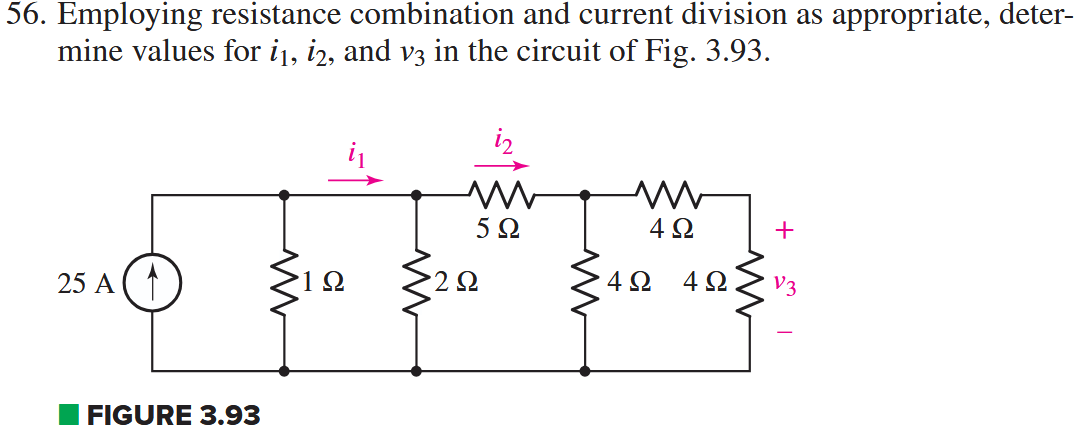
\includegraphics[width=0.8\textwidth]{3-56.png}
\end{figure}
\vspace{-1em}

\section*{3.60}
\vspace{-3.5em}
\begin{figure}[H]
    \centering
    
\includegraphics[width=0.8\textwidth]{3-60.png}
\end{figure}
\vspace{-1em}

\section*{3.61}
\vspace{-3.5em}
\begin{figure}[H]
    \centering
    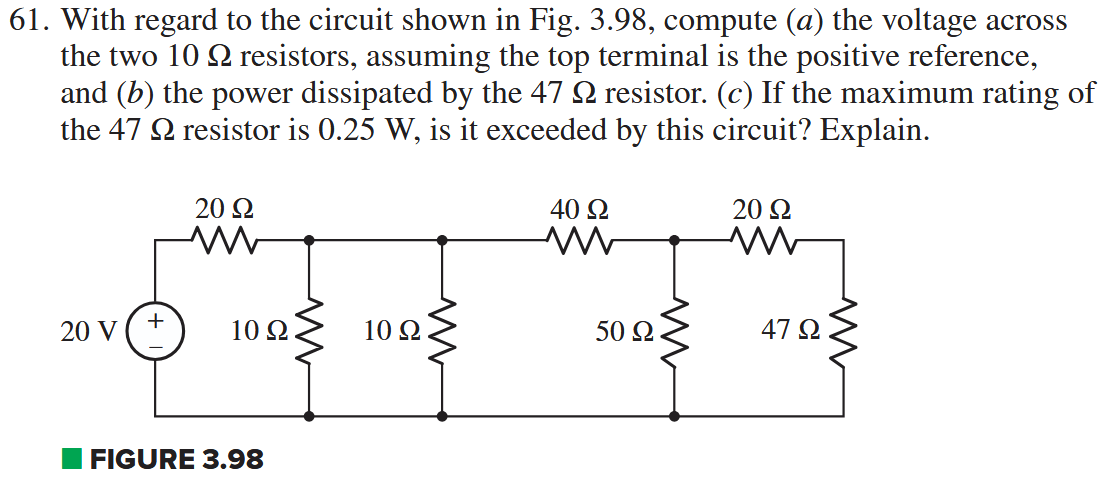
\includegraphics[width=0.8\textwidth]{3-61.png}
\end{figure}
\vspace{-1em}

\end{document}